%% Load document class fithesis2
%% {10pt, 11pt, 12pt}
%% {draft, final}
%% {oneside, twoside}
%% {onecolumn, twocolumn}
\documentclass[12pt,final,oneside]{fithesis2}

%% Basic packages
\usepackage[english]{babel}
\usepackage{cmap}
\usepackage[T1]{fontenc}
\usepackage{lmodern}
\usepackage[utf8]{inputenc}
\usepackage{graphicx}

%% Additional packages for colors, advanced
%% formatting options, etc.
\usepackage{color}
\usepackage{microtype}
\usepackage{url}
\usepackage{cslatexquotes}
\usepackage{fancyvrb}
\usepackage[small,bf]{caption}
\usepackage[plainpages=false,pdfpagelabels,unicode]{hyperref}
\usepackage[all]{hypcap}

%% Fix long URLs in DVIs
\usepackage{ifpdf}

%% Source code highlight

\usepackage{floatrow}
\usepackage[chapter]{minted}
\usemintedstyle{trac}
%get caption above code
\floatsetup[listing]{style=Plaintop}
%caption style    
\captionsetup[listing]{format=listing,labelfont=white,textfont=white, singlelinecheck=false, margin=0pt, font={bf}}
%fancyvrb frame
\renewcommand{\listingscaption}{Example}


\DeclareGraphicsExtensions{.pdf,.png,.jpg}

\ifpdf
\else
  \usepackage{breakurl}
\fi

%% Packages used to generate various lists
\usepackage{makeidx}
\makeindex

\usepackage[xindy]{glossaries}
\makeglossary

%% Use STAR and CIRCLE signs for nested
%% itemized lists
\renewcommand{\labelitemii}{$\star$}
\renewcommand{\labelitemiii}{$\circ$}

%% Title page information
\thesistitle{Integration of JBoss Undertow HTTP server with Apache Camel project}
\thesissubtitle{Master's thesis}
\thesisstudent{Dávid Šimanský}
\thesiswoman{false} %% Important when using Slovak or Czech lang
\thesisfaculty{fi}  %% {fi, eco, law, sci, fsps, phil, ped, med, fss}
\thesislang{en}     %% {en, sk, cs}
\thesisyear{Autumn 2014}
\thesisadvisor{Mgr. Marek Grác, PhD.}

%% Beginning of the document
\begin{document}

%% Front page with a logo and basic thesis information
\FrontMatter
\ThesisTitlePage

%% Thesis declaration (required)
\begin{ThesisDeclaration}
  \DeclarationText
  \AdvisorName
\end{ThesisDeclaration}

%% Thanks (optional)
\begin{ThesisThanks}
 I would like to thank to my supervisor Mgr. Marek Grác, Ph.D. and my technical supervisor from Red Hat Czech, s.r.o, Mgr. Jiří Sedláček,  for providing constant feedback during the preparation of this master's thesis.
 
Many thanks goes to all my other colleagues from Red Hat that expressed their valuable thoughts and helped to make this thesis better.   
\end{ThesisThanks}

%% Abstract (required)
\begin{ThesisAbstract}
The purpose of this master's thesis is to design and develop new Camel component by integrating two open-source project Apache Camel and JBoss Undertow. This new component will act as HTTP provider in the Camel integration framework.
\end{ThesisAbstract}

%% Keywords (required)
\begin{ThesisKeyWords}
Apache Camel, Undertow, Java NIO, XNIO, integration framework, web server, component 
\end{ThesisKeyWords}

%% Beginning of the thesis itself
\MainMatter

%% TOC (required)
\tableofcontents

%% Thesis text structured using
%% chapters, sections, subsections, etc.
\chapter{Introduction}
We, the people of the Information Age, are surrounded with technologies providing us information or making our lives easier. We benefit from machine-processed informations and in many areas we are totally dependent on computers controlling the environment around. The IT segment is fast paced and innovative. New technologies emerge every day, but sometimes lifetime is as short as the development time. Nevertheless, there are still many information systems based on various programming languages up and running, containing numerous priceless data. The improvements made in networking and the Internet over the years changed the view we anticipate information systems. Nowadays we see need for connecting them together to benefit from code already created and running to provide input data or business logic. Although not every system has the right interface to be interconnected and is ready or designed to operate in complex environment. All of that creates the base ground from which integration frameworks raise to satisfy already existing demand.

The demand to enable interoperability across platforms, programming languages, data formats and interfaces. Main goal of an integration framework should be to simplify the complexity of integration and also unify the management. Also it can not be hard to adopt to actually bring benefits to users rather then discourage them with difficult learning process.

Apache Camel project\cite{camel-web} is one of the integration frameworks used for above mentioned purpose. It is open source based, developed under Apache with a great help from community. The main advantage of Camel is its modularity, for every new communication protocol just a new component needs to be added. That enables Camel to keep the core lightweight and stable to provide the right tools for every given scenario.

 The purpose of this thesis is to create new Camel  component. It should act as HTTP\footnote{HTTP - Hypertext Transfer Protocol} provider in Camel. This component should benefit from yet another open source project JBoss Undertow\cite{undertow-web}. Undertow is web server, written in Java\cite{java-web} from scratch and based on non-blocking principles. This component was required through community process as a new feature to incorporate into the distribution. The reasons might not be clear at first as there already are several other HTTP components available in the Camel distribution. Similarly to Camel, Undertow is lightweight and easy to embed. It is also used in Wildfly application server. The chapter 2.6.2 contains performance comparison of various HTTP server implementations. From the result it can be seen that among Java based web servers Undertow is constantly placing in the top three. The Undertow is also gaining popularity inside the open source community. It is still relatively young project that might have bright future. The thesis creates base for the future cooperation of Camel and Undertow projects.   
 
Based on community given approach the new component is named Camel Undertow.   
 
 The thesis itself is divided into five thematic parts. The first chapter contains introduction and motivation with the overview of the following chapters.
 
 The second chapter introduces all the technologies used in implementation. The text is not detailed to provide just the most important facts and link to detailed sources for further reading.

Analysis and design are summarized in the third chapter. It contains diagrams and reasons to support design decisions.

The next chapter illustrates implementation of the new component created for this thesis.

The last chapter is conclusion of the work.

\chapter{Technologies}
This chapter introduces technologies that are used for implementation of Camel Undertow component. Every sub-chapter consists of description and typical uses cases, where the specific technology excels.

\section{Apache Camel}
Apache Camel is open source rule-based mediation framework implemented in Java. The core of the framework is formed around the theory of EIPs\footnote{EIP - Enterprise Integration Pattern} by Gregor Hohpe and Bobby Wolf\cite{eip}. It creates base layer in integration efforts across various applications, e.g. in stand alone routing, communication of web services, enterprise messaging solutions or full integration platforms (also known as ESB\footnote{ESB - Enterprise Service Bus}) like Apache ServiceMix, JBoss Fuse or JBoss Fuse Service Works. Based on previously mentioned fact, Camel is not an enterprise service bus on its own, for instance it does not provide container support or messaging broker. It aims to be lightweight, easy to adopt and extendable for developers. There is also no complex class hierarchy or APIs rather emphasizing the focus on integration tasks\cite{camel-in-action}.

\subsection{Fundamental principles of Camel}

The idea behind Camel is to get the maximum potential from the theory of EIPs and to efficiently minimize the lines of source code needed to implement integration scenarios. Therefore a convention over configuration approach is used to describe the task in declarative way by domain-specific language (DSL).  The Camel's DSL creates common way for developers to integrate the applications which is easy to learn and afterwards apply, regardless of transport protocols, delivery format, payload encoding or endpoints connectors. There is no canonical format or assumption of data format directly hardcoded in the framework. This fact gives developers working on integration task no limiting condition, literally any kind of system could be merged together.

\subsection*{Routing and mediation engine}
Routing engine enables users to define custom rules for routing messages, acceptance strategy for sources sending to endpoint, also add processors on the way to modify the payload and finally decide to which destination message is delivered.

\subsection*{Domain-specific language}
The format of DSL varies by the preference or experience of individual. It is not bound to Java language only, whatever developer likes Java, XML, Groovy, Ruby or even Scala.

\begin{listing}[ht]
	\inputminted[]{java}{sources/java_dsl_example.java}
	\caption{Java DSL definition of route}

\end{listing}

\begin{listing}[ht]
	\inputminted[]{xml}{sources/xml_example.xml}
	\caption{XML definition of route }

\end{listing}

\begin{listing}[ht]
	\inputminted[]{java}{sources/scala_example.java}
	\caption{Scala definition of route }

\end{listing}

\subsection*{Modular implementation}
The next key feature, that supports wide adoption of the framework in integration world, is modularity. The Camel can be easily extended to  consume or to produce data to endpoint. Out of the box it comes with handful of components to start with, called camel-core including bean, file, log, mock. Following the structure given by the framework and extending core classes developers are able to provide solution to whatever unique system you could imagine. On top of that, there are many more developed by Apache community and third-parties\footnote{List of components - http://camel.apache.org/components.html}. The most common integration scenarios can be served by already existing components to integrate JMS\footnote{JMS - Java Messaging Service}, web services (SOAP\footnote{SOAP - Simple Object Access Protocol} or REST\footnote{REST - Representational State Transfer}), database connections, filesystem resources or mobile push services.

\subsection*{Automatic type converters}
Built-in automatic type converter is able to work with more than hundred and fifty class types out of the box. For most of the scenarios the converter is available, but also custom ones can be implemented easily. This feature is one of the most favorite in the community. It can by easily triggered by the following example \ref{converter} which demonstrates that method used to retrieve body takes as a parameter desired return type, the converter is used without any further interaction from the calling code.

\begin{listing}[ht]
	\inputminted[]{java}{sources/converter.java}
	\caption{TypeConverter invocation}
	\labe{converter}
\end{listing}

\subsection*{Convention over configuration}
The ease of configuration is another fundamental principle to enable developers focus on important tasks rather than learning number of complicated configuration options. Endpoints can be configured directly in route definitions with URI options as the example \ref{uri-option} demonstrates.
\begin{listing}[ht]
	\inputminted[]{java}{sources/uri.java}
	\caption{URI options configurations}
	\label{uri-option}
\end{listing}


\subsection*{Lightweight from the start}
From the first line it is designed to be undemanding and resource friendly. Core library of Camel has about 1.6 MB in total with minimum of third party dependencies.  Embedding the framework is straightforward regardless of target platform, which can be web application, Spring container, OSGi bundle or various cloud platforms. 

\subsection{Message types}
Various kind of data types are transported in Camel's routes as Messages. There are two main classes that create abstraction of messages, Message\footnote{Class of org.apache.camel.Message} and Exchange\footnote{Class of org.apache.camle.Exchange}.
%% linebreak
\\ \\
Message object represents data carried in routes from sender to receiver in system's communication. It consists of body, headers and optional attachments. Every Message has unique identifier (UID). UID format is not strictly given by Camel and is dependent on linking protocol. If the protocol doesn't have UID scheme available, there is generic generator provided by framework.

Headers are pairs of key and value, based on very same principle as in HTTP protocol. They contain identifying informations as UID, sender, receiver, type of content, encoding and authentication information.

Body represents payload or content of the message. It has generic Object type to store any kind of content. Acceptance of body type by receiver has to be ensured by application embedding Camel, either by transformation inside the route or by using of automatic type converter.
%% linebreak
\\ \\
Exchange object is a message's container for routing and encapsulates Message. It supports message exchange patterns (MEPs). Property to define messaging style can be set in exchange pattern, either one-way or request-response. One-way is called \textit{InOnly} and is used for example in JMS, when sender does not require response. Request-response is defined as \textit{InOut}, most typical example is HTTP transport, when client needs to receive reply.
Overview of Exchange's content:
\begin{itemize}
\item Exchange ID - unique identifier of Exchange
\item MEP - type of messaging style
\item Exception - in case of error exception is stored
\item Properties - various Camel properties for routing, can be also edited by developers
\item In message - input request message
\item Out message - output response message, only if the pattern is \textit{InOut}
\end{itemize}



\subsection{Architecture overview}
The following part will introduce core parts of Camel's design starting from the top. The figure 2.1 illustrates the overview to easier understands the runtime of CamelContext.

\begin{figure}[!h]
\centering
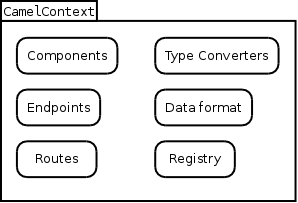
\includegraphics[width=0.5\linewidth]{images/camelContext.png}
\caption{Overview of CamelContext}
\end{figure}

  


\subsection*{Camel context}
Camel context is commonly referenced as container, which keeps everything together and provides services during runtime. List of most important services:
\begin{itemize}
\item components - used in application, they can be added on the fly 
\item endpoints
\item routes
\item type converters
\item data formats
\item registry - for beans look up. Default is JNDI registry\footnote{JNDI registry - Java Naming and Directory Interface http://docs.oracle.com/javase/8/docs/technotes/guides/jndi/jndi-rmi.html}. If Camel is combined with Spring or OSGi container, it uses native registry mechanism for the deployment
\end{itemize}

\subsection*{Routers and routing}
Routes are one of the core concepts used in this framework. The route holds definition of input source and output target. Simple route can be defined as a chain of processors. Every route is absolutely identified by its unique ID, has exactly one input source that is tied to input endpoint and one or many targets.

Routing works under the hood and is not visible to users. It ensures proper routing from the sender to receiver without issues.

\subsection*{Processor}
The name is self explaining. Processor is responsible for processing incoming exchange, creation, modification or removal of payload and headers. Many processors can be chained together and are invoked by the rules defined in route. Most of built-in processors are implementation of EIPs, as stated previously, Camel supports most of integration patterns.\footnote{EIPs in Camel - http://camel.apache.org/eip.html} Users has possibility to implement custom processors and add them to the route.   

\subsection*{Component}
Components add modularity to Camel, they are main extension point. Their task is to be factory of endpoints. The detailed overview of creating new component will be given later in subchapter 2.2. 

\subsection*{Endpoint}
Endpoints represent sender or receiver on the one end of the message channel. Endpoint is configured by URI, during runtime Camel looks up an endpoint by its URI. Format of URI has three important parts: scheme, context path and options. The scheme contains information about component to be used. In this thesis our scheme is called \textit{undertow}. Context path identifies the location of endpoint, similarly to web page address. Finally the options part is used to deliver specific configuration for component.

One of the key tasks of endpoint is to be factory for creating consumer (receiver) and producer (sender), that can be used in route to get the data flowing.  

\subsection*{Consumer}
As already stated, consumers can be seen as receivers of messages. It is the starting point of every route, where the message is sent, wrapped with headers and added to exchange. Exchanges created by consumer are afterwards processed in defined chain of processors. 

There are two types of consumers, event-driven and polling consumers. They could be also called passive and active consumer. Event-driven consumer is in EIP referred as asynchronous receiver, represents client-server communication strategy. It listens on messaging channel and waits for incoming message. 

Polling consumer is active and synchronous, received message has to be processed before polling for another one. Basically, it fetches messages from the source. In Camel the scheduled polling consumer can be defined to check for message in time interval.  


\subsection*{Producer}
Producer is used to create and send a message to an endpoint. It is responsible for creating message and mapping the message content for the endpoint. In this component it creates HTTP request and acts as HTTP client.


\section{Component development}
Modularity feature is ensured by components as it was already mentioned. They are used to extend Camel and adapt to new integration tasks and add new protocols support without necessity to edit the core implementation of the framework. This part contains the main principles that should be followed to create custom component.

 To speed up the development, it is recommended to use Maven archetype as a base for the new component.\footnote{Maven archetypes - http://camel.apache.org/camel-maven-archetypes.html} The generated skeleton is fully functional HelloWorld example, which is generating dummy messages in intervals. The next step should be naming the component. Component name must be unique among existing components, because it is used in the first part of URI to identify it. List of components distributed with Camel can be found on official web pages stated earlier. 
 
 The hierarchy of classes that need to be implemented is quiet simple. There are four main classes that together create Camel component, Component, Endpoint, Producer and Consumer. The names are of course self explaining. The Component class is on top for creating and managing the underlying Endpoint class. Moving to the Endpoint class, it's responsible for creating Producer or Consumer as needed. The custom implementation can extend particular Default-prefixed classes and leverage from the default framework code rather than writing everything from scratch. Extending existing classes ensures following of main principles\cite{camel-cookbook}.
 
\subsection*{Component class}
This class acts as factory of endpoints. Therefore it must implement at least \textit{createEndpoint()} method. The best to achieve it is by extending DefaultComponent. It also contains all parameters that can be set with URI options. Parameters can be annotated with \textit{@UriParams} and then set through reflection by Camel.

 \subsection*{Endpoint class}
 Endpoints are factored by Component class. Its purpose is to manage Producers and Consumers. There should be creation method for both of them. Not every component has to have Producer and Consumer, when it is not needed. If the option is not supported appropriate exception should be thrown to inform user.
 
 \subsection*{Consumer class}
 Through Consumer the message enters the route. There are several handy classes in default implementation for event-driven and polling consumers. There are no major restriction how to implement this class. In the code UndertowConsumer represents web server that is started by the definition from route and waits for incoming HTTP request to send them down to the route. 
 
\subsection*{Producer class}
To be able to send messages outside there has to be Producer class implementation. It is used to establish connection, marshal the data and send them to particular target. \texit{UndertowProducer} in this thesis acts as HTTP client for sending requests.

\section{Integration in action}
DZone\footnote{DZone - http://www.dzone.com/} web site claims to be online community and collection of resources for technology professionals. The web site is well know in community of IT professionals and has outstanding reputation for serving the high quality content. The integration is one of the most prominent topics that DZone focuses on. In 2014 they performed update to its overview research among consumers of integration technologies. It provided overview of usage the integration in practice, recommendations from the top engineers and solution architects and comprehensive comparison of most used solutions. The findings were published in free e-book called \textit{DZone Guide to Enterprise Integration}\cite{dzone}. This part will summarize the key aspects from the research. The relevance of this research is supported by the sample of respondents, most of them have technical background, mainly developers and team leads. The programming language used is Java in 94\% of cases.

\subsection*{State of Integration}
The integration scenarios are typically covered by integration framework combined with message queues or ESB.  
In the beginning ESBs were based on Messaging-Oriented Middleware or required Java EE containers for runtime. They gained on popularity with the increased usage of web services, which were quickly integrated. ESB focuses on covering wide range of scenarios, supported with the tools out of the box. It ties together multiple endpoints, where central broker does all the heavy lifting of routing, transforming and managing\cite{esb}.

On the other hand integration frameworks like Apache Camel or Spring Integration benefit mainly from outstanding support of enterprise integration patterns. They can be paired with message queues and other frameworks to enrich with missing features to be comparable with full ESBs.

 Previously mentioned can be viewed as traditional well know and verified approach. On the other hand new emerging trend supported by innovative technological companies seems to be microservices. The idea behind microservices is fundamentally different from ESBs. There is no central point or smart mediator that routes communication, but they rather emphasize smart endpoints and fast transfer channel with minimum of features. Each microservice represents one logical or business feature of the system, it shares common principle with processes in Unix-like operating systems to do single thing right. The communication channels are not tied to process, but they use web services or remote calls.

In conclusion there might be an upcoming shift to more decentralized solutions called microservices. Although most of the scenarios can be still well served with the integration frameworks and ESBs.

\subsection*{Leader Board}
The DZone's research provides interesting statistics on usage of technologies. 
The most popular technology among respondents is Spring Integration\footnote{Spring Integration - http://projects.spring.io/spring-integration/} (42\%), closely followed by the Camel framework (38\%). In the category of ESBs, the winner is Mule ESB\footnote{Mule ESB - http://www.mulesoft.org/what-mule-esb} (16\%), then WebSphere ESB\footnote{WebSphere - http://www-03.ibm.com/software/products/en/wsesb} (15\%) and Oracle ESB\footnote{Oracle ESB -  http://www.oracle.com/technetwork/middleware/service-bus/} (13\%). In conclusion, lightweight integration frameworks are more popular taking 63\%.

 When ESBs and message queues are compared it ends slightly better for the ESBs. The most popular messaging is ActiveMQ\footnote{Apache ActiveMQ - http://activemq.apache.org/} (46\%) that beats low-latency providers like ZeroMQ\footnote{ZeroMQ - http://zeromq.org} or IronMQ\footnote{IronMQ - http://www.iron.io/mq}. 
 
 The conclusion based on the above mentioned numbers can be made that developers tend to choose lightweight modular solutions rather than the full stack of unnecessary features.




  
 \section{Java NIO}
Java NIO represents New IO, an alternative implementation to the standard IO API used in the Java language. The key differences include reading data from channels into buffers or vice versa, whenever the standard API uses streams of bytes or chars. The other are non-blocking IO instead of typical blocking IO, when thread is blocked until read or write is completed\cite{java-nio}.

Non-blocking approach means that the execution thread is not blocked, therefore is not waiting for completion of read or write operation, instead it redirects it to channel and buffer and continues to operate. Afterwards if the data are available in the buffer even partially, the thread can process it. The write operation acts the same way, data are stored in buffered and written to channel, in the meantime the executing thread can handle some other operation.

The idea is that a single thread can manage multiple input and output operations. The thread is not blocked by reading from one stream, nevertheless do something useful during meantime.

The Channels are similar to Stream approach with some differences. Data are read or written to Buffer. They are also bi-direction in contrast to Stream which can be used just for reading or writing. Operations performed on Channels are asynchronous. All those differences come from the usage of Buffer where data are stored from Channel and not processed directly as in Stream.

The Buffers are used for storing data from Channels as mentioned above. In simple, Buffers are wrappers for blocks of memory with methods to access the memory easier.  

The Selector is a kind of object monitoring multiple channels for events to further extend capability of single thread. The usage of Selector gives a possibility to use one IO thread to process data from multiple Channels, every time the Channel is ready to be read or written Selector will notify the working thread.

Emphasizing NIO approach developers are able to lower the resource consumption of the application, especially thread pools to handle multiple IO connections and memory usage, because every new thread is associated with some portions of belonging memory. There is ongoing discussion if the multithread or the single thread is better approach. The single thread has benefit of less overhead, meaningful resource allocation and overall lowering the complexity of application, where the thread synchronization and possible deadlocks are not present anymore.  

\section{XNIO}
XNIO is community project developed under JBoss, which provides framework abstraction over low level Java NIO and brings simplification over working with Channels, Buffers and Selectors. It extends NIO to support multicast socket and non-socket IO. The project web page claims that XNIO also opens the door to non-obvious optimizations.

One of the most important features of XNIO framework is its unique API, that combines both IO approaches, blocking and non-blocking to bring the best to users. The benefits of low latency of blocking IO with throughput and performance of non-blocking.

  Undertow web server is fully based on XNIO framework under the hood, that is one of the reason why developers embedding Undertow can easily switch between blocking and non-blocking processing of incoming requests\cite{xnio-doc}.

\section{Undertow}

Undertow is a flexible performant web server written in Java, providing both blocking and non-blocking API, which are based on XNIO, the abstraction over Java NIO introduced in previous subchapter.

Undertow has a composition based architecture that allows you to build a web server by combining small single purpose handlers. That gives you the flexibility to choose between a full Java EE servlet 3.1 container, or a low level non-blocking handler, to anything in between.

Undertow is designed to be fully embeddable, with easy to use fluent builder APIs. Undertow’s lifecycle is completely controlled by the embedding application\cite{undertow-doc}.

Overview of key features:
\begin{itemize}
\item Lightweight - the core jar is under 1 MB, runtime taking up about 4 MB of heap
\item HTTP upgrade support - multiple protocols over HTTP
\item Web Socket -  full support, including JSR-356
\item Servlet 3.1 support 
\item Embeddable - fully runnable from inside the application
\item Flexible - just the right amount of functionality for the task can be used by chaining handler's together
\end{itemize}

\subsection{Embedded server}
As stated above, Undertow is fully embeddable. There are two ways how to achieve it. The more simple way is  to use builder API and set various properties as handlers, listeners, context paths and listening ports. The second approach is to manually assemble the whole server using XNIO and listener classes directly. Using builder API is sufficient for the purpose of this thesis.

There is no container, that is required to start. Embedded web server is managed by embedding application, also usage and chaining of handlers is under control of the application. 

\subsection{Performance benchmark}

The web development company, TechEmpower, regularly updates benchmark results of popular web servers and frameworks. By the results presented on the web pages filtered by language, Undertow is listed as the fastest amongs Java based web servers, in the underlying figure 2.2 is presented the example from results. For the full chart, metrics and enviroment setup follow the link on the company web pages.\footnote{Web server benchmarks - http://www.techempower.com/benchmarks/}

\begin{figure}[!h]
\centering
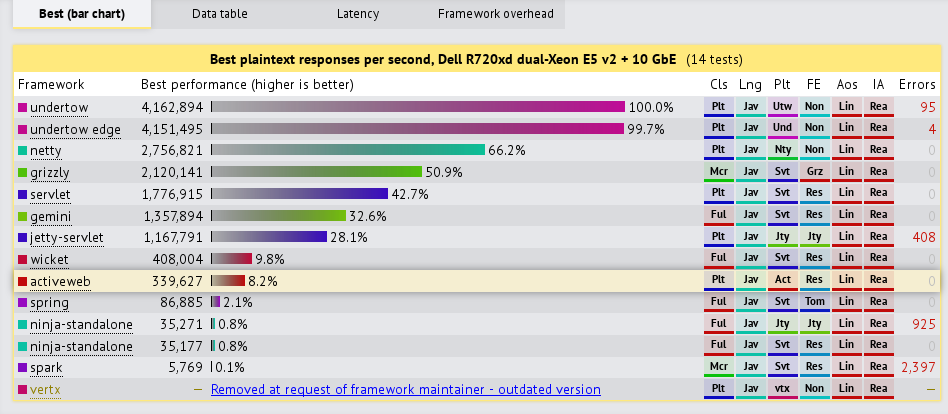
\includegraphics[width=1\linewidth]{images/undertow_benchmark.png}
\caption{Performance comparison of web servers\cite{perf}.}
\end{figure}

\newpage

\section{Similar HTTP components}
The official Camel distribution already provides several components that have very similar functionality in comparison to Camel Undertow and are considered as HTTP provider components. The following part  will summarize the main differences between Camel HTTP, Camel Servlet, Camel Netty, Camel Netty HTTP and Camel Jetty. The last subsection will discuss the motivation for developing Camel Undertow components. Those lines are author's subjective through and summaries. 

\subsection{Camel HTTP}
Camel HTTP is one of the core components. It supports only usage of producer, which acts like HTTP client. Therefore it cannot be used as input in the route definition. The implementation leverages Apache HttpClient library\footnote{Apache HttpClient  - http://hc.apache.org/httpclient-3.x/} to produce requests. When there is no special requirement for producing HTTP request, this component should be absolutely sufficient for most basic scenarios. 

\subsection{Camel Servlet}
Camel Servlet on the other hand provides support for input message, which is sent to Java servlet published by the endpoint. As the servlet container Tomcat web server is used in the implementation. The full route with consumer and producer endpoints can be achieved by combining Servlet and HTTP components.

\subsection{Camel Netty and Netty HTTP}
This component is implemented on top of Netty framework. The Netty project is also NIO based and should enable quick development of network application. Both blocking and non-blocking sockets are supported. It provides capability for both types of endpoint bind to TCP\footnote{TCP - Transmission Control Protocol} or UDP\footnote{UDP - User Datagram Protocol} protocol. This component should be used if the direct access to above mentioned protocols is needed.

Netty HTTP is extending the parent Netty component and add HTTP transport support. 

\subsection{Camel Jetty}
Another HTTP provider component that is based on Jetty server implementation. The Jetty library contains also client support. Therefore both types of endpoint are also supported. Jetty itself is popular as a servlet container and component leverages this fact. The Consumer is implemented in similar fashion and exposes CamelServlet object, which creates input for a route.

\subsection{Camel Undertow - motivation}
It may be confusing why we need another HTTP component, when there are so many already implemented and capable to satisfy user's needs. The easiest answer is, because we can. If there is another web server implementation, why don't create yet another Camel component for it. 

Certainly the answer is not so simple. The Camel user's community is wide and divergent. Some of them are satisfied with components coming from distribution. Another group might prefer writing its own component for specific task.

Camel Undertow is based on non-blocking approach to IO operations. It is written from scratch, performance numbers are also quiet promising. It is emerging new technology. There is no high demand for Camel Undertow component yet, but in few years the story may be completely different. Undertow might become very popular and dominant among Java web server implementations. Right now it is more a possibility than a necessity. 

 


\chapter{Analysis and Design}
This part of the thesis will benefit from all the facts written in previous chapters and provide software analysis for new component. Not every part of software analysis is needed for the purpose of this thesis. Development of components is restricted and follows the skeleton given by the framework. The analysis starts with identifying of requirements which this new component should support. Data flow diagram (DFD) is used to illustrate the context of incoming and outgoing messages and processing inside Camel.  Afterwards the design decisions made on the analysis follows.

\section{Requirements}
The main purpose of the thesis defined by the assignment is to integrate JBoss Undertow project with Apache Camel project. The outcome of the integration should be new component that could be used as a web server (HTTP provider). This new component is also required by community in the Apache's Jira.\footnote{Camel Undertow - https://issues.apache.org/jira/browse/CAMEL-6577}

As already mentioned in previous chapter, there is plenty of other components available that can server to the same purpose as Camel Undertow. Why to develop another one? The answer is pretty simple to provide diversity to end users. Undertow is  an emerging technology in the community of Java developers. So far it looks very promising as high performance and super lightweight web server. The world of HTTP servers is mainly focused on performance numbers and results of Undertow are in many ways impressive in regard that it is still pure Java implementation. Also it's gaining on popularity due to the fact that it is used in Wildfly\footnote{Wildfly - http://www.wildfly.org/} application server since version 8.0. In conclusion the fundamental features of Camel and Undertow seem very coherent to tie them together. 

The thesis assignment does not provide any detailed listing of requirements. Therefore the following requirements are based upon analysis of similar components acting as HTTP providers and default features for every component:

\subsection{Consumer}
\begin{itemize}
\item ability to create Consumer as HTTP web server 
\item user defined context path and listening port
\item define allowed request methods
\item secured access options through HTTPS
\item DSL and Spring support
\end{itemize}

\subsection{Producer}
\begin{itemize}
\item send HTTP requests to defined target 
\item DSL and Spring support
\end{itemize}

\section{Data flow diagram}
DFD is used to depict the data flow incoming to Consumer and outgoing from Producer.

The figure \ref{dfdconsumer} shows Consumer message flow. It is needed to map the incoming HTTP request to Exchange object. Every part of HTTP request should be copied to Exchanges (payload, headers, method type, etc.) to provide users with additional information they could benefit from.
\begin{figure}[!h]
\centering
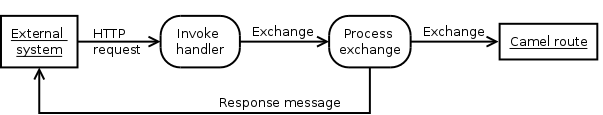
\includegraphics[width=1\linewidth]{images/consumer.png}
\caption{DFD illustrates Consumer receiving message.}
\label{dfdconsumer}
\end{figure}

Producer message flow is shown in figure \ref{dfdproducer}. The process is reverse to Consumer part. From the Exchange back to HTTP request. 
\begin{figure}[!h]
\centering
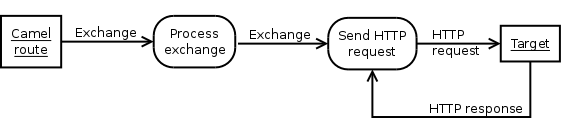
\includegraphics[width=1\linewidth]{images/producer.png}
\caption{DFD illustrates Producer sending message}
\label{dfdproducer}
\end{figure}

\section{Use case diagram}
The Use case diagram does not depict the user actors, because Camel Endpoints mainly communicate with applications or APIs.  

\begin{figure}[!h]
\centering
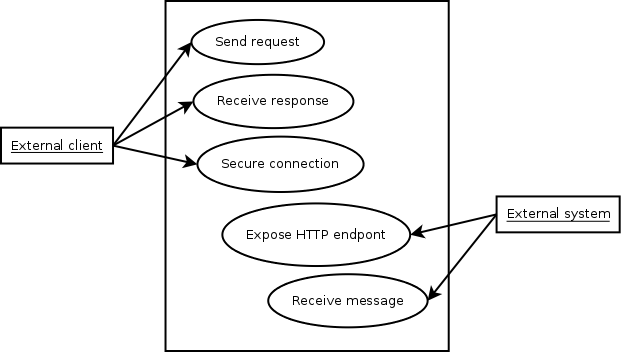
\includegraphics[width=1\linewidth]{images/useCase.png}
\caption{Use case depicts communication through component.}
\end{figure}

\section{Design decisions}
The design of the component has to follow guidelines given by the Camel framework mentioned in chapter 2.2. Therefore the class hierarchy and structure is already clear.

Undertow will be embedded through builder API and the whole server lifecycle will be controlled by the component. During the research of client capabilities it was found out that client classes are not suitable for general HTTP client. It was designed to be used in reverse proxy. This fact was confirmed by the lead developer, Stuart Douglas.\footnote{Undertow-dev mailing list - http://lists.jboss.org/pipermail/undertow-dev/2014-December/001072.html} In his response, he mentioned that the client is 100\% non-blocking and not thread safe. There was discussion in the community about adding a thread safe wrapper, but it is not implemented yet. For the completeness of the component the client classes in the Producer will be used. The implementation will follow points given by Stuart in the email. 

Although, users should be warned in the documentation that Producer part is not ideal and should be used with caution. The Producer is exchangeable to other HTTP Producers from components mentioned in chapter 2.6 to ensure proper behavior.



\chapter{Implementation}
 The goal of this thesis is to integrate Apache Camel and JBoss Undertow to create new Camel Undertow component. This chapter summarizes the source code and implementation of Camel Undertow component.

The source code for was implemented in Java programming language with regard to restriction of components development mentioned in previous chapters. During the development coding conventions and best practices gained in various courses at Faculty of Informatics were leveraged.

Listing of version used in the source code:
\begin{itemize}
\item Java 1.7
\item Apache Camel 2.14.0
\item Undertow 1.1.1.Final
\end{itemize}
\section{Class diagram}
The full exported class diagram can be found in appendix A.2. In the following sections partial diagrams to depict single class will be used.

\section{UndertowComponent class}
\begin{figure}[ht!]
\centering
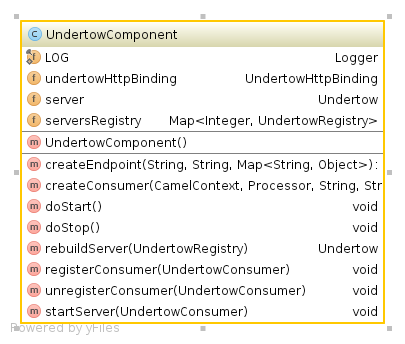
\includegraphics[width=0.6\linewidth]{images/undertowComponent.png}
\caption{UndertowComponent class in more detailed vies.}
\end{figure}

This class is a starting point of the implemented component. It extends \textit{HttpComponent} to build on the core of Camel code. Its purpose is to be factory of endpoints. Therefore \textit{createEndpoint()} method is the most important one.

This method is straightforward. First it reads all the configuration URI parameters and removes them to prevent mismatching them as query parameters. After the incoming URI is cleaned, the Endpoint URI is parsed from the rest.

There is also support for \textit{RestConsumerFactory} to extend configuration of routes and options in REST-style DSL. \footnote{Camel REST DSL - http://camel.apache.org/rest-dsl.html} For this purpose only one new method has to be added, \textit{createConsumer()}. In this method the REST configuration is parsed and belonging endpoint is created.

The class also holds configuration of running web server. This fact enables usage of multiple Endpoints with different paths on the same port, but sharing same base configuration. By the base configuration is meant host, port and SSL support. If those three conditions are not satisfied and therefore route is considered misconfigured another route on the same port cannot be started.

\subsection{UndertowRegistry}
 \begin{figure}[!h]
\centering
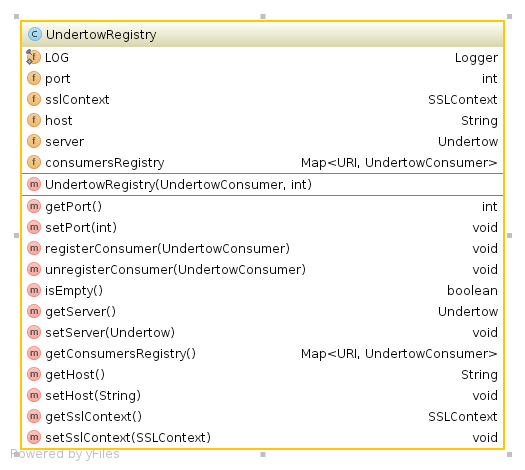
\includegraphics[width=0.6\linewidth]{images/undertowRegistry.png}
\caption{UndertowRegistry class in more detailed vies.}
\end{figure} 

The \textit'{UndertowRegistry} class represents registry of running web servers and belonging Consumers. This utility class is only used inside of \textit{UndertowComponent} class. Through the registry Component is able to access server instance, register and unregister new Consumers. It provides handful of methods to provide convenient access.

This class was added due to the fact that workflow of Builder API is not suitable for runtime modifications. Once the server is built, the Builder instance can not be retrieved anymore from server instance. Although dynamic modification of server configuration was needed, either by storing object of \textit{Undertow.Builder} or by adding configuration object from which the Builder can be created. That is the reason to implement \textit{UndertowRegistry} class. As mentioned previously the ability to modify server runtime brings benefit of sharing port across Endpoints. 

\section{UndertowEndpoint class}

The Endpoint represents a factory for creating Consumers and Producers. This class holds configuration parameters parsed in \textit{UndertowComponent.createEndpoint()}. Primitive types parameters are annotated with \textit{@UriParam} to allow setting through Java Reflection API. 

The methods \textit{createProducer()} and \textit{createConsumer()} are self explaining. Another important one is \textit{createExchange()} which takes \textit{HttpExchange} from web server as input and converts it to Camel Exchange.  The main part of this logic is done in \textit{toCamel()} from class \textit{DefaultUndertowHttpBinding}. The binding class provides support for converting incoming HTTP messages to Camel messages and vise versa.

\begin{figure}[!h]
\centering
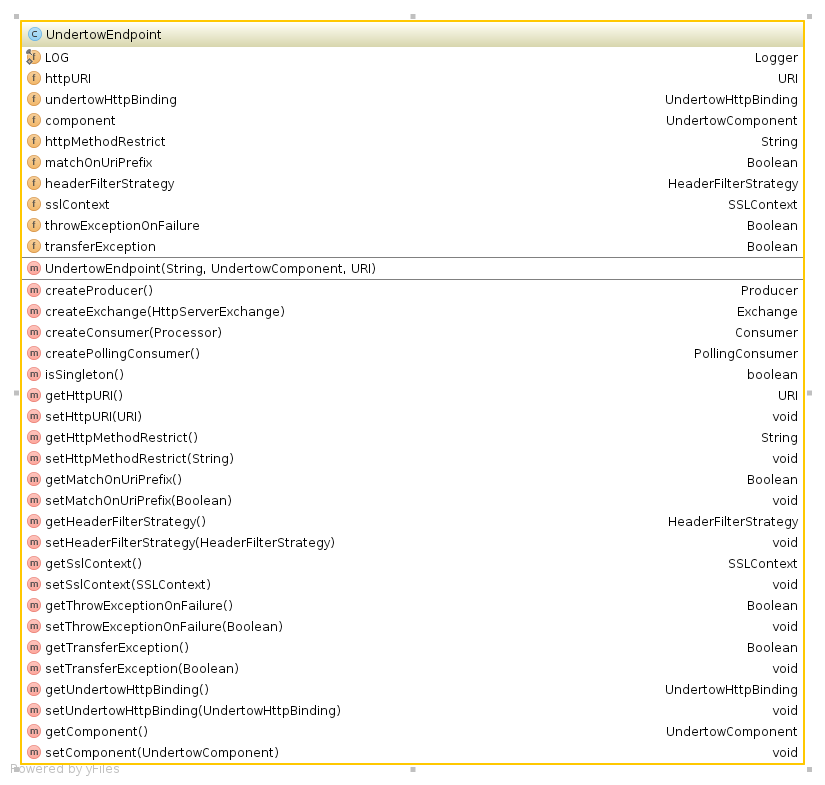
\includegraphics[width=0.7\linewidth]{images/undertowEndpoint.png}
\caption{UndertowEnpoint class in more detailed view.}
\end{figure}

\subsection{Parameters}
Most of the configuration parameters are self explaining. Although in the underlying listing the basic description is given to avoid any confusion.

List of parameters:
\begin{itemize}
\item httpUri - holds the full URI as defined in route
\item undertowHttpBinding - the instance of actual binding tied to the Endpoint
\item httpMethodRestrict - list of comma separated HTTP methods that can be used to access Consumer
\item matchOnUriPrefix - boolean value which determines if exact or prefix matching of path should be used 
\item headerFilterStrategy - the instance of HeaderFilterStrategy, by default the strategy from HTTP component is used
\item sslContext - provides configuration for the web server
\item throwExceptionOnFailure - boolean value whether the exception should be thrown
\item transferException - boolean value if the exception should be send back in response 
\end{itemize}


\section{UndertowConsumer class}

\begin{figure}[ht!]
\centering
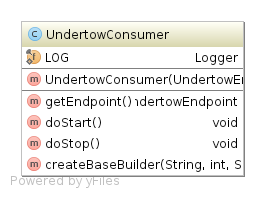
\includegraphics[width=0.43\linewidth]{images/undertowConsumer.png}
\caption{UndertowConsumer class in more detailed view.}
\end{figure}

Essential classes for the component functionality. This class itself starts the Undertow web server and allows it to be used as entry to the Camel route. 

There are two possible approaches how to handle incoming request. Java servlet, in particular \textit{CamelServlet} or its extension, can be exposed to process the incoming messages and send them to route. First prototype was implemented in that fashion. Although it was discarded later due to the fact that Undertow doesn't provide straight way to access servlet instance once deployed to the server. The instance is need during processing to retrieve the request and create particular Exchange. This approach didn't provided the desired amount of control over the processing of incoming request.

On the other hand Undertow is easily extensible with custom handlers. Therefore all the logic of processing the HTTP request is moved to \textit{HttpCamelHandler}, but it still might be considered as a part of Consumer.

The web server is started through methods in \textit{UndertowComponent} class as already mentioned in section 4.2. When new Consumer needs to be added \textit{UndertowComponent.registerConsumer()} is invoked and afterwards \textit{UndertowComponent.rebuildServer()} to reflect change in configuration. Configuration of running server is rebuilt and server instance restarted. Upon \textit{doStop()} invocation the Consumer is unregistered from \textit{UndertowRegistry}, the method also checks if there are any other Consumers left to shutdown whole server and release allocated port.





\subsection{HttpCamelHandler class}
Implementing of custom handlers for Undertow is straightforward. The custom handler needs to implement \textit{HttpHandler} interface which contains only one method \textit{handleRequest()}. Through this method the handler gets to \textit{HttpExchange} object which contains request and response channels, headers and request method type. 

The processing of request has few partial conditions to meet to finally proceed to Camel Exchange. If the \textit{OPTIONS} method is received, the handler returns allowed methods. It checks for restricted methods from configuration and rejects all requests that do not follow the given restriction. If the request method can contain payload (POST, PUT), the request channel is opened to retrieve the body of message, otherwise payload is ignored for other methods.\cite{http}

The Exchange is created through \textit{createExchange()} method in Endpoint implementation. The whole \textit{HttpExchange} is used as input. During the Exchange creation \textit{toCamelMessage()} is invoked from the default HTTP binding to copy and filter required headers. The default HTTP binding is provided by class \textit{DefaultUndertowHttpBinding} which implement \textit{UndertowHttpBinding} interface. Conversion of HTTP request to Message benefits from automatic type converter feature. The body is extracted as array of bytes and directly set to Message object, the type converter works under the hood without direct invocation in the binding method. The binding can be changed to custom implementation specified in URI option to modify the behavior, copied headers, etc. When the Exchange is created the Processor can kick off and process it.

 Finally after processing of Exchange, the response can be retrieved and send back to requesting client. The standard return code is 200 and body from Camel Message is included, if there is any. In case of error, the return code is 500 and the exception is transferred, if the option parameter is not set to false. The response is created by method \textit{toHttpResponse()} that copies headers and returns body as \textit{Object}. The body is afterwards converted to \textit{ByteBuffer} and sent to requesting client.

\section{UndertowProducer class}
The implementation of Producer can be considered experimental and is not recommended for usage. The Undertow client classes are not designed to be used as general HTTP client. As mentioned in previous chapter, they are not thread safe and provides bridge in reverse proxy.

For end users it is recommended to use Camel HTTP or Camel Netty HTTP component as Producer provider.

The actual source code benefits from the recommendations given by Stuart Douglas. It is capable of creating HTTP request from the Message and sending it to target, afterwards receive and read the response. The conversion from HTTP to Camel Message is provided by another handy methods from binding class \textit{DefaultUndertowHttpBinding}.

\begin{figure}[ht!]
\centering
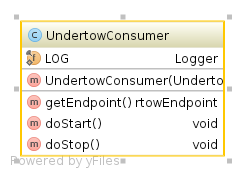
\includegraphics[width=0.5\linewidth]{images/undertowProducer.png}
\caption{UndertowProducer class in more detailed vies.}
\end{figure}

\section{UndertowHttpBinding}
The binding interface and its implementation \textit{DefaultUndertowHttpBinding} represent the key aspect of how the Messages are created from HTTP requests and vice versa. It is used in Producer and Consumer classes. 

It is capable of processing HTTP request in a manner that all headers are extracted and stored in Camel Message, filtered by the given strategy. It is also responsible for reading payload if the requesting method is allowed to have one. Finally the incoming Message is returned to be used in the route.

After processing of the Message is done the binding also maps the response back to HTTP response through the similar process as described above.

The reverse steps are done for the creation of HTTP request in Producer's code. The Camel message is transformed to request and send, when the HTTP response is received, it is stored back to Camel Message.

\begin{figure}[ht!]
\centering
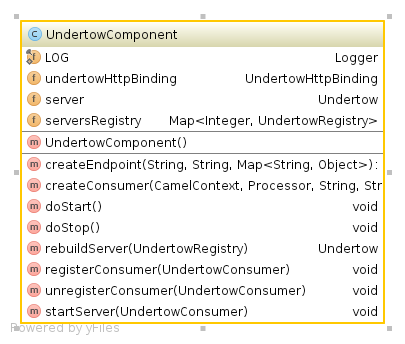
\includegraphics[width=0.6\linewidth]{images/undertowComponent.png}
\caption{UndertowHttpBinding interface in more detailed vies.}
\end{figure}


\section{Miscellaneous classes}
There are two additional classes that provides support methods.

\textit{ExchangeHeaders} is a copy of \textit{Exchange} class fields that contains header names. Instead of returning them as \textit{String}, this class returns \textit{HttpString} for Undertow to minimize conversion of header names on various places.

\textit{UndertowUtil} contains just method for simple appending headers to map.

\section{Unit tests}
The unit tests leverage \textit{CamelTestSupport} classes that provides lot of useful method and mock Endpoints to properly test components. The structure of unit tests follow convention used in Camel project. Every test class represents scenario and has descriptive self-explaining name to be clear for the outside user.

\section{Simple performance comparison}
The newly created component was compared in simple test with two other components. The comparison was performed between Undertow, Jetty and Netty HTTP. The results supports the conclusion the Undertow is built to be fast and outperform the opponents.

\begin{figure}[ht]
\centering
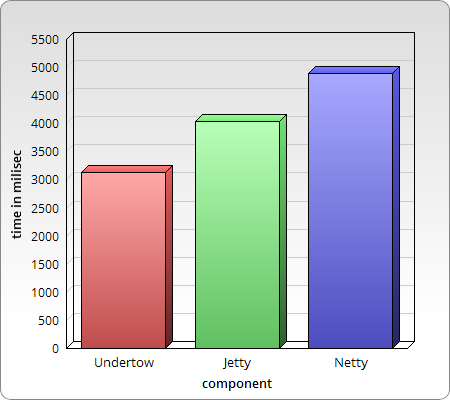
\includegraphics[width=0.49\linewidth]{images/1K.png}
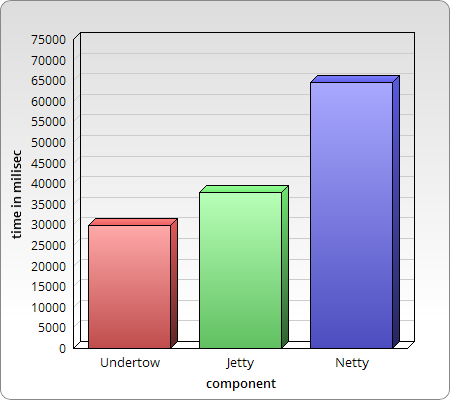
\includegraphics[width=0.49\linewidth]{images/10K.png}
\caption{Execution time graph for 1000 and 10 000 requests.}
\end{figure}

The metric used was simple to demonstrate the possible testing approach. For more comprehensive results a special tool could be used to generates requests and measure numbers, for example PerfCake\footnote{PerfCake - https://www.perfcake.org/}
 The scenario was run ten times and average execution time value was calculated afterwards. Test scenario class is called \textit{UndertowPerfComparisonTest} and can be found in unit tests subdirectory. During the first cycle thousand of request was sent, the next cycle the number of request was increased to ten thousand. To further improve the comparison and relevance of results dedicated performance hardware or lab should be used as this simple comparison was performed just on standard laptop.

\begin{table}[h]
\begin{tabular}{|c|c|c|l|}
\hline
\multicolumn{1}{|l|}{No. of requests} & \multicolumn{1}{l|}{Undertow} & \multicolumn{1}{l|}{Jetty} & Netty                        \\ \hline
1000                                  & 3141 ms                       & 4045 ms                    & \multicolumn{1}{c|}{4892 ms} \\ \hline
10 000                                & 29 755 ms                     & 37 792 ms                  & 64 532 ms                    \\ \hline
\end{tabular}
\caption{Results in numbers.}
\end{table}


\section{Examples of usage}
There are two examples of route definition included in the attachment. They demonstrates the configuration and usage in Java DSL and Spring API. The whole example project can be run by Camel Maven plugin\footnote{Camel Maven plugin - http://camel.apache.org/camel-run-maven-goal.html}. This plugin simply runs the Camel context defined in a project. The instructions to run this particular project: 
\begin{itemize}
\item First it is needed to build the component code in camel-undertow directory
\textit{mvn clean install}
\item Navigate to camel-example-undertow directory and compile the example itself \textit{mvn compile}
\item The last step \textit{mvn camel:run}
\end{itemize}

The above mentioned steps are also included in ReadMe file with the example source code.

\begin{listing}[ht]
	\inputminted[]{java}{sources/dsl-example.java}
	\caption{Java DSL}
\end{listing}

\begin{listing}[H]
	\inputminted[]{xml}{sources/spring-example.xml}
	\caption{Spring API}
\end{listing}






\chapter{Conclusion}
The primary goal of this master's thesis was to integrate JBoss Undertow HTTP server and Apache Camel project. Under integration is meant design and development of a new Camel component. This new component should be used as a web server (HTTP provider) in the integration framework. As part of this thesis unit test and example of usage in DSL and Spring API should be delivered. Furthermore author should cooperate with community, study Camel component development process and investigate the Undertow implementation.

The outcome of this master's thesis is Camel Undertow component. The new component can be used as HTTP provider to act as Consumer in the route. 

As an attachment the source code of the component is included. This component was requested by the community, it will be submitted to Apache Camel project as pull request for the review. The latest source code is hosted on GitHub\footnote{GitHub repo - https://github.com/dsimansk/camel-undertow}. The computer software in general is never absolutely perfect. Therefore there is a possibility that issues and bugs will be found in future during usage or code reviews.  All the found issues can be reported through GitHub tools or even be fixed by pull request from the community. The previous also applies for enhancement requests.

The implementation part of this thesis includes the whole source code of the new component. The skeleton was generated by Maven archetype. The main part of work is represented by embedding the Undertow to the Camel. The mechanism for the managing lifecycle and storing configuration of the web server was created. The server is started by Camel itself. Furthermore, the binding between HTTP messages and messages transferred inside the Camel routes was needed. The component provides both Endpoint types, Consumer and Producer with the limitation illustrated in following paragraph. The detailed description of implemented classes can be found in chapter 4.

During the research work it was found out that Undertow client libraries are not suitable for implementing a general purpose HTTP client.
There was already a discussion in the community about this topic as mention in chapter 3. It should be merged to this component to harden the Producer implementation. The following fact implies that Producer implementation is not stable and should not be used outside of tech preview scope. It can be replaced by any other provider mentioned in this thesis. Although for the completeness purpose the Producer code is included. The actual implementation will probably vary in future based on the code changes inside Undertow.

For the future development, the main goal is to harden the Producer part once the Undertow client is done by the community. Other requirements submitted from users and community will be added after consideration. Bug fixes should be done as soon as possible, it is highly dependent on current situation and capacity.

New component implementation is well documented in various sources online and offline. The Camel community has vital and extensive community that provides many examples, answers on StackOverflow\footnote{StackOverflow - http://stackoverflow.com/questions/tagged/apache-camel} and comprehensive documentation. As mentioned in chapter 2 there are also other very similar components to look for. The Undertow community is definitely much smaller. There is not so many materials available as for Camel definitely. Although almost all questions are answered by the authors of code themselves. The Undertow project is still finding its place under the Sun, the number of users and adopters raises. In a few years it might be dominant web server among Java based implementations. With the increasing interest will also the number of resources available grow significantly. 




%% Lists of tables and figures, glossary, etc.
%%\printindex
%%\printglossary
%%\listoffigures
%%\listoftables

\begingroup
\def\tmpchapter{0}
\renewcommand{\chaptername}{}
\renewcommand{\thechapter}{}
%%\addtocontents{toc}{\setcounter{tocdepth}{-1}}
\chapter{References}
\renewcommand{\chapter}[2]{}% for other classes

\bibliographystyle{plain}
\bibliography{references}

\begin{thebibliography}{}
\bibitem{camel-web} APACHE. \textit{Apache Camel} [online]. 2004- [cite 2014-12-12]. Available at: \url{http://camel.apache.org/}

\bibitem{undertow-web} JBOSS. \textit{JBoss Undertow} [online]. 2014- [cite 2014-12-12]. Available at: \url{http://undertow.io/index.html}

\bibitem{java-web} ORACLE. \textit{Java} [online]. \copyright{} 2004- [cite 2014-12-12]. Available at: \url{http://www.java.com/}

\bibitem{eip} HOHPE, Gregor and WOLF, Bobby. \textit{Enterprise integration patterns}. Boston: Addison-Wesley, c2003, li, ISBN 978-0321200686.
				
\bibitem{camel-in-action} IBSEN, Claus and ANSTEY,Jonathan. \textit{Camel in Action}. Greenwich, Conn.: Manning, c2011, xxxi, ISBN 
19-351-8236-6.

\bibitem{camel-cookbook} CRANTON, Scott and KORAB, Jakub. \textit{Apache Camel Developer's Cookbook}.  Birmingham: Packt publishing, c2013, ISBN 9781782170303.

\bibitem{dzone} DZONE RESEARCH. \textit{Guide to Enterprise Integration} [online]. 2014- [cite 2014-12-14]. Available at: \url{http://www.dzone.com/research/guide-to-enterprise-integration}

\bibitem{esb} THOMAS, Anne. \texit{https://www.gartner.com/doc/1405237/enterprise-service-bus-definition} [online]. 2007 - [cite 2014-12-14]. Available at: \url{https://www.gartner.com/doc/1405237/enterprise-service-bus-definition}

\bibitem{java-nio} ORACLE. \textit{Java NIO} [online]. 2014- [cite 2014-12-12]. Available at: \url{http://docs.oracle.com/javase/7/docs/api/java/nio/package-summary.html}

\bibitem{xnio-doc} JBOSS. \textit{XNIO Documentation Developer's Guide} [online]. 2014- [cite 2014-12-12]. Available at: \url{https://docs.jboss.org/author/display/XNIO/Developer%27s+Guide}

\bibitem{undertow-doc} JBOSS. \textit{JBoss Undertow Documentation} [online]. 2014- [cite 2014-12-12]. Available at: \url{http://undertow.io/documentation/}

\bibitem{perf} TECH EMPOWER. \textit{Web Framework Benchmarks - Round 9}. 2014- [cite 2014-12-16]. Available at: \url{http://www.techempower.com/benchmarks/#section=data-r9&hw=peak&test=json&l=3k}

\bibitem{http} NETWORK WORKING GROUP. \textit{Hypertext Transfer Protocol -- HTTP/1.1
} [online]. 1999- [cite 2014-12-03]. Available at : \url{https://www.ietf.org/rfc/rfc2616}
\end{thebibliography}

\endgroup
%% Additional materials
\appendix

\chapter{Appendix}

\section{Contents of included CD}
\begin{itemize}
\item master's thesis in PDF
\item source code of the thesis in \LaTeX
\item source code of Camel Undertow component
\item examples
\end{itemize}

\newpage

\section{Class Diagram}
\begin{figure}[ht!]
\centering
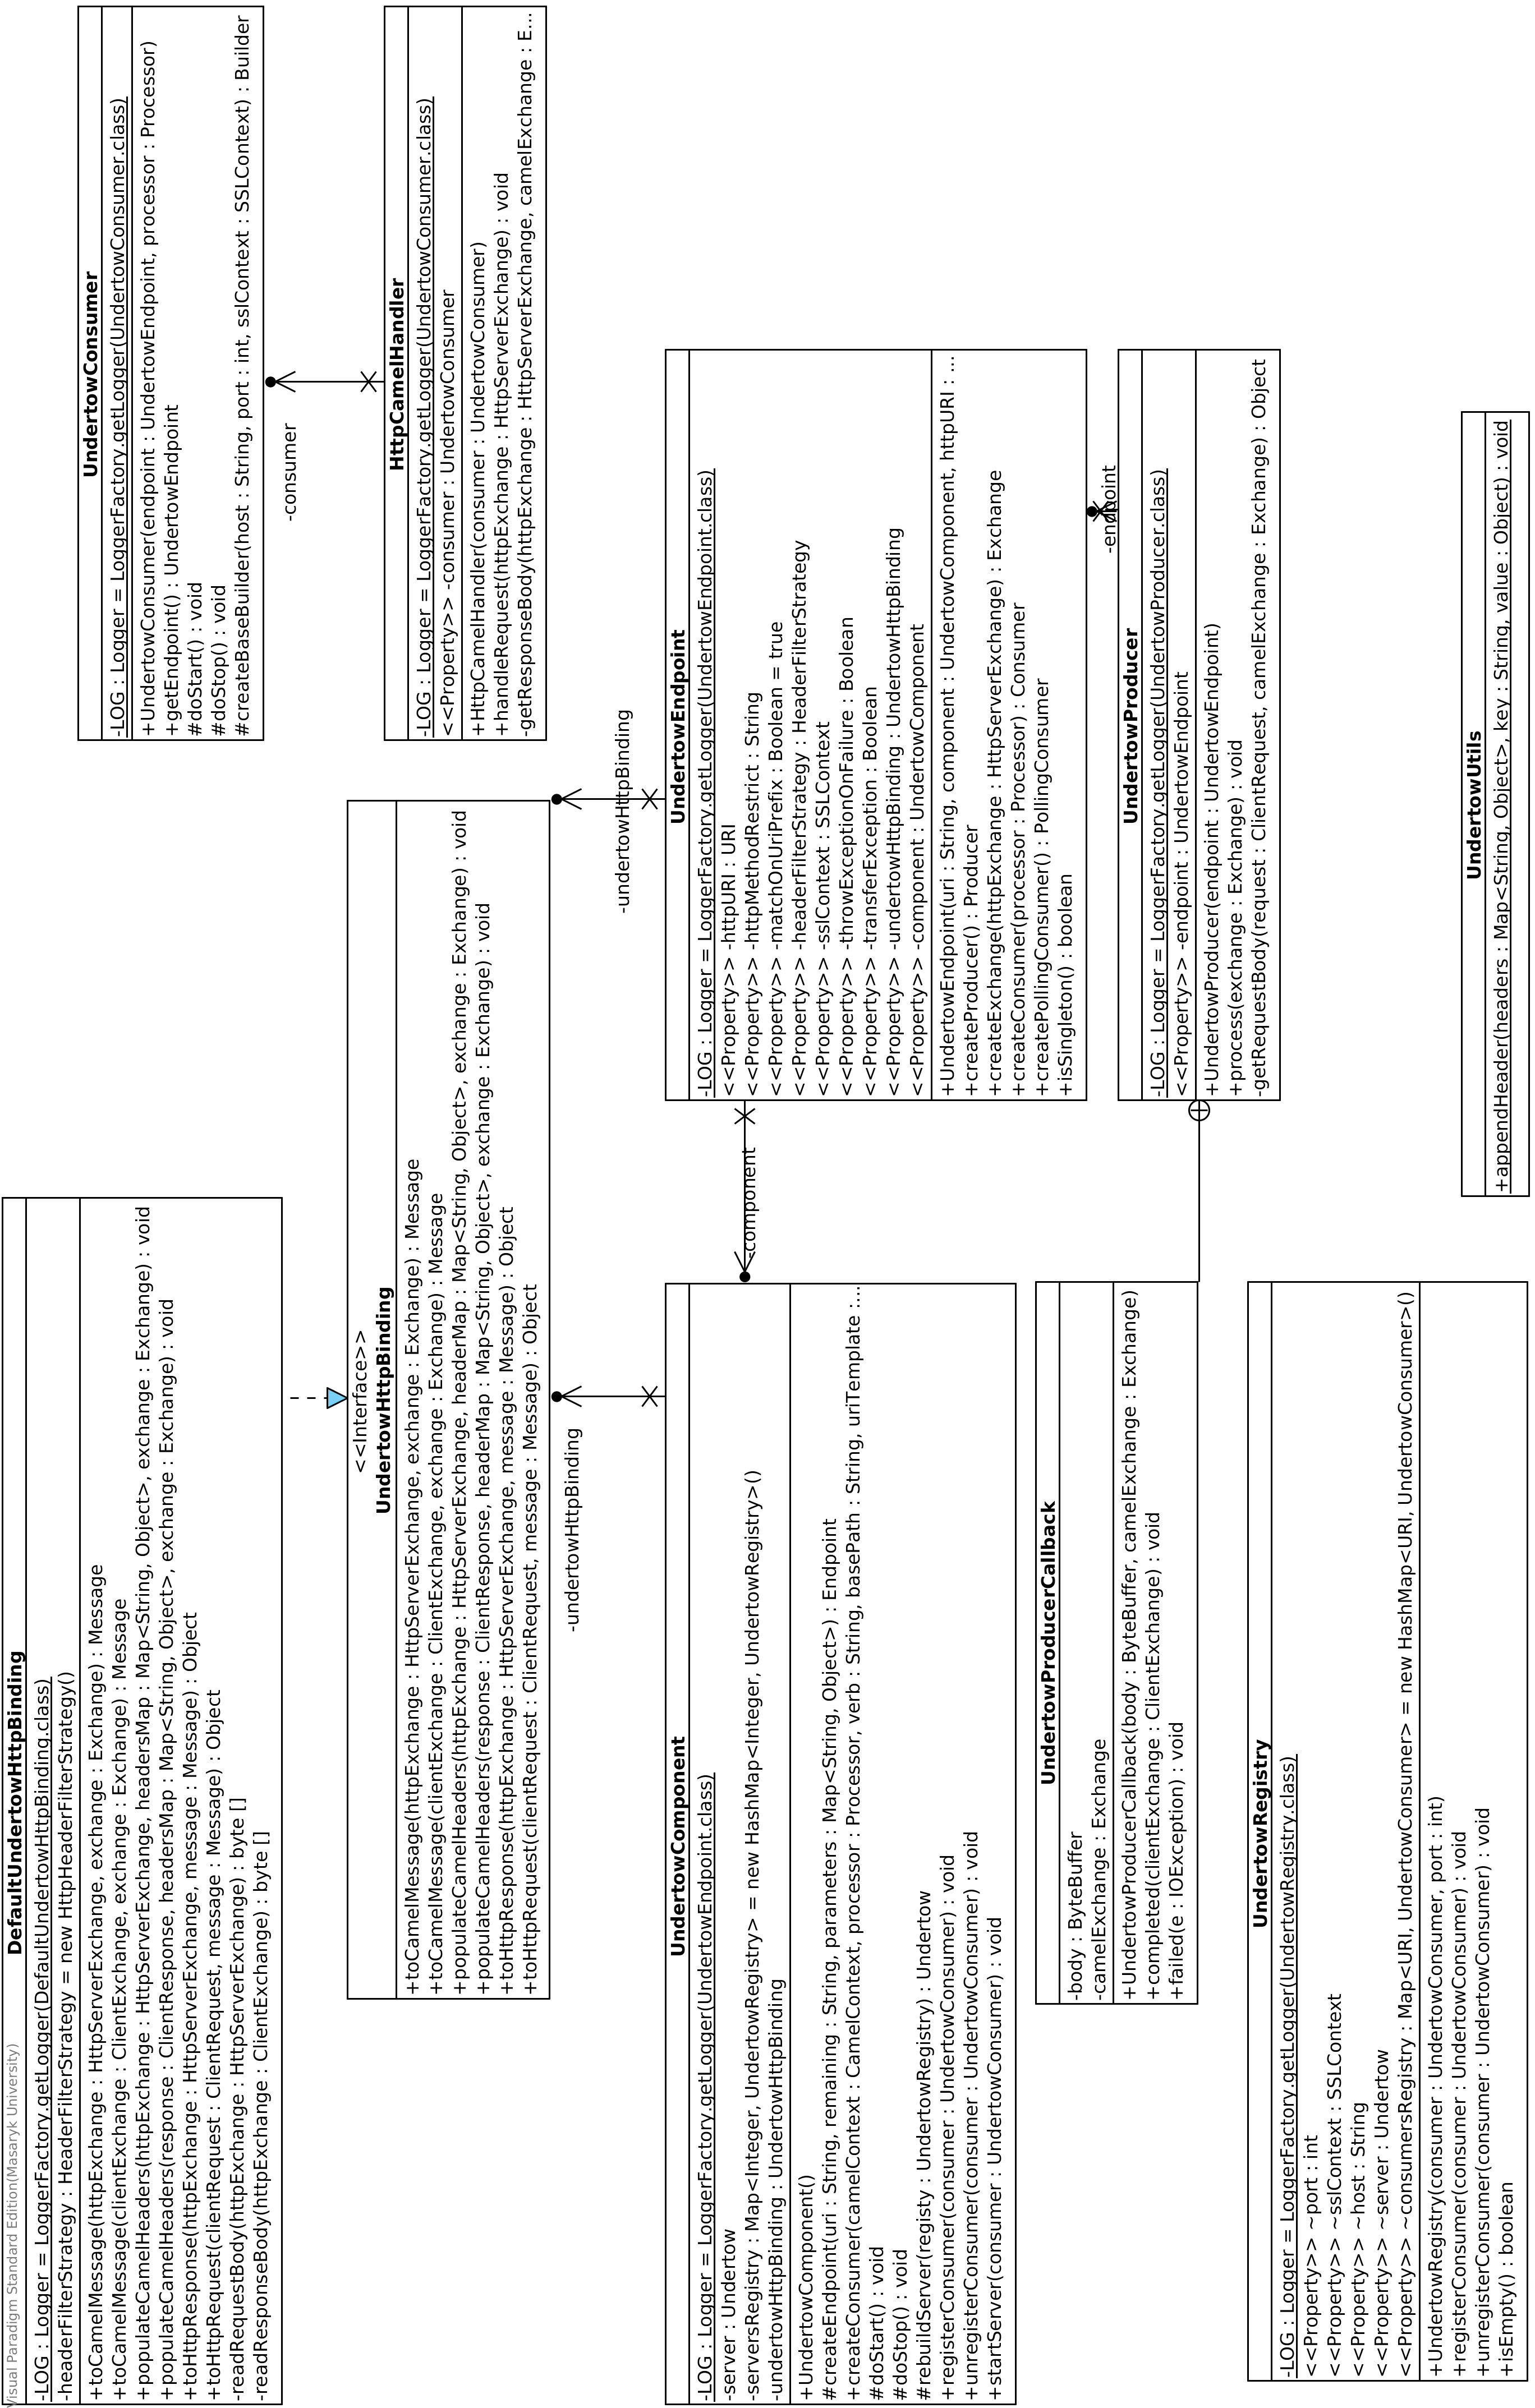
\includegraphics[width=0.85\linewidth]{images/classBig.png}
\end{figure}

%% End of the whole document
\end{document}